\documentclass[11pt,a4paper]{article}
\usepackage[margin=2.2cm]{geometry}
\usepackage{graphicx}
\usepackage{booktabs}
\usepackage{xcolor}
\usepackage{tcolorbox}
\usepackage{hyperref}
\usepackage{caption}
\usepackage{float}
\usepackage{fancyhdr}
\usepackage{titlesec}
\usepackage{enumitem}
\usepackage{tabularx}
\definecolor{navy}{HTML}{1F3A5F}
\definecolor{teal}{HTML}{2A9D8F}
\definecolor{red}{HTML}{C8553D}
\definecolor{grey}{HTML}{8D99AE}
\hypersetup{colorlinks=true,linkcolor=navy,urlcolor=teal}
\titleformat{\section}{\Large\bfseries\color{navy}}{\thesection}{0.6em}{}
\titleformat{\subsection}{\large\bfseries\color{navy}}{\thesubsection}{0.5em}{}
\pagestyle{fancy}\fancyhf{}
\fancyhead[L]{\small\color{grey}Zinger market making: results, capital and economics}
\fancyhead[R]{\small\color{grey}22 October 2026}
\fancyfoot[C]{\small\thepage}
\setlength{\parskip}{0.5em}
\newtcolorbox{callout}[1][]{colback=teal!8,colframe=teal,boxrule=0.6pt,arc=2pt,left=8pt,right=8pt,top=6pt,bottom=6pt,#1}
\newtcolorbox{warn}{colback=red!7,colframe=red,boxrule=0.6pt,arc=2pt,left=8pt,right=8pt,top=6pt,bottom=6pt}
\captionsetup{font=small,labelfont=bf,labelformat=simple,labelsep=period}
\graphicspath{{../figures/}}
\newcolumntype{Y}{>{\raggedright\arraybackslash}X}

\title{\textcolor{navy}{\textbf{Zinger Market Making on Polymarket}}\\[0.3em]
\large What is working, what is not, and the economics per \$100}
\author{Research record \\ Paper trading and public market data only}
\date{22 October 2026 (UTC)}

\begin{document}
\maketitle
\thispagestyle{empty}

\begin{callout}
\textbf{Status and risk disclosure.}\\
No order has been placed and no money spent; every figure is a simulation on live public data.
\textbf{What is working:} reward capture in every quoted market, 29 of 40 liquid markets net positive on unseen data (+\$44.61 per day on \$9,874), low-fill settings positive 95\% of the time, and small budgets (\$100--\$1,000) positive in the capital simulation.
\textbf{Overall portfolio result:} across all 40 liquid markets the out-of-sample result was $-$\$42.44 per day ($-$0.33\%), because three large adverse moves outweighed the winners. Section~\ref{sec:neg} covers this in full. Real capital remains conditional on the gates in Section~\ref{sec:gates}.
\end{callout}

\section{Positive results}

\subsection{Reward capture works in every quoted market}
\begin{figure}[H]\centering
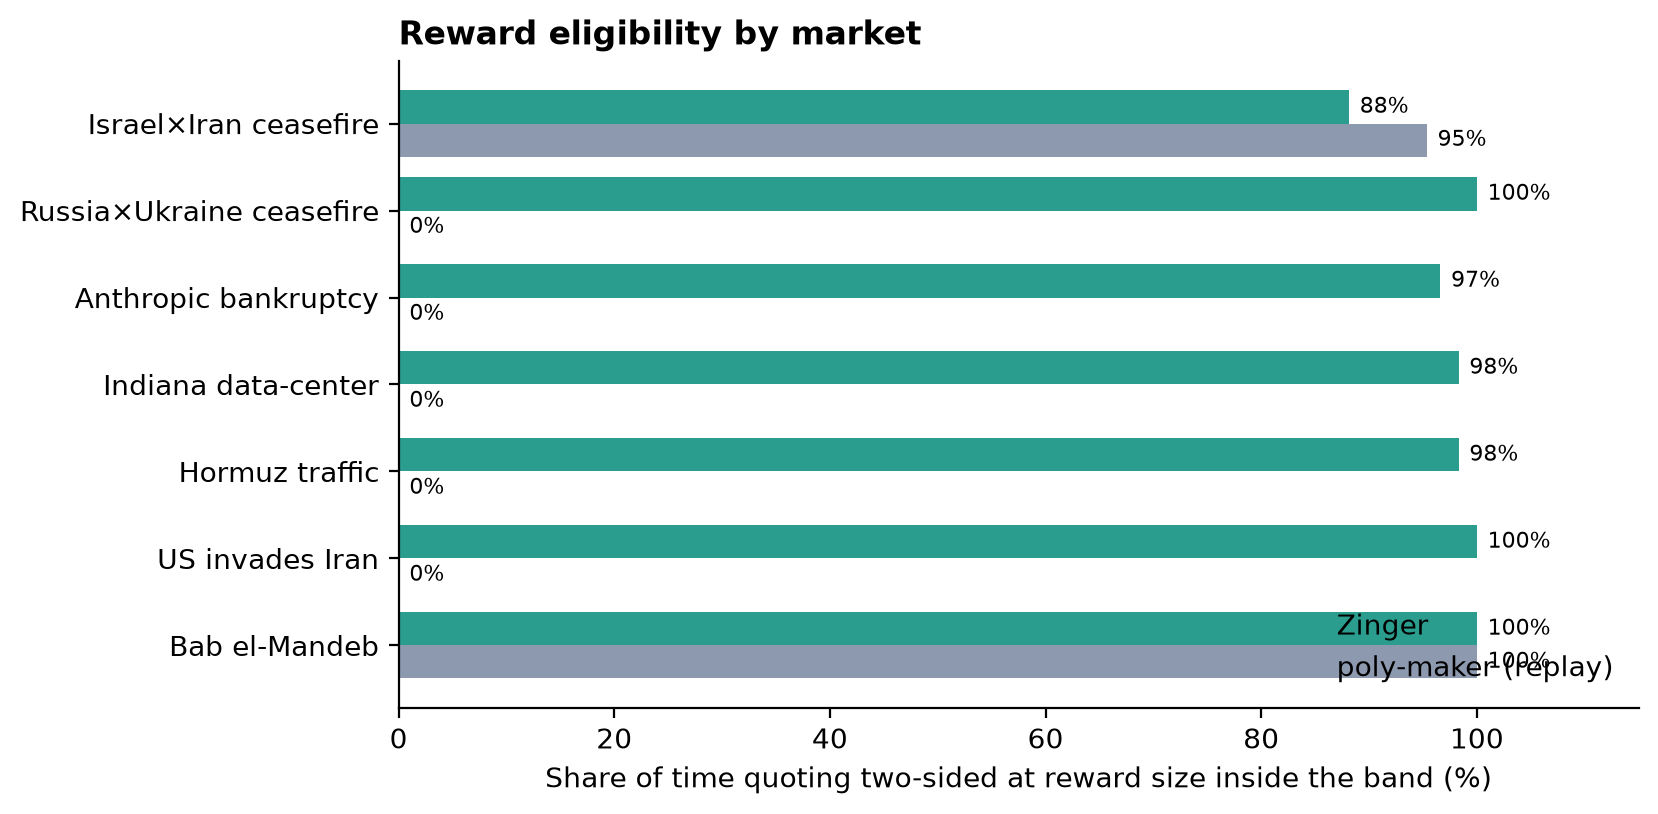
\includegraphics[width=0.48\linewidth]{bench2_eligibility}\hfill
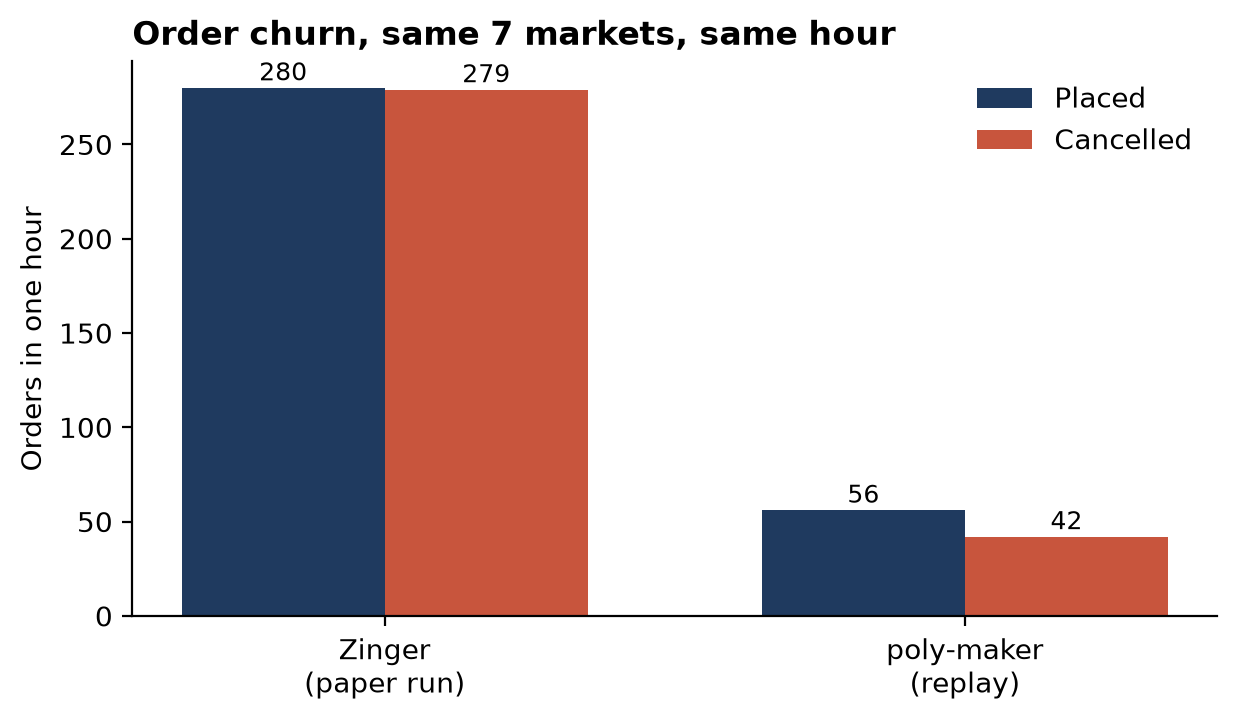
\includegraphics[width=0.48\linewidth]{bench1_churn}
\caption{Left: Zinger quoted two-sided at reward size inside the band in 7 of 7 markets (an open-source bot managed 2 of 7). Right: orders placed and cancelled in the same hour.}
\end{figure}
\begin{table}[H]\centering\small
\begin{tabular}{@{}lrr@{}}
\toprule
Measure & Before fixes & After fixes \\
\midrule
Time with stale books & 72\% & 0.7\% \\
Markets scoring rewards & 1 of 7 & 7 of 7 \\
Orders kept vs placed (one hour) & 38 placed & 47,004 kept, 280 placed \\
Liquid-market projected reward, 24 h & --- & \$10.4--\$14.1/day, steady \\
\bottomrule
\end{tabular}
\caption{Engineering fixes turned an unreliable quoter into one that rests orders and qualifies for rewards continuously.}
\end{table}

\subsection{29 of 40 liquid markets were net positive on unseen data}
Settings were chosen per market on the first 12 hours of a 24-hour recording and scored on the second 12 hours, after a deliberately pessimistic fill cost.
\begin{figure}[H]\centering
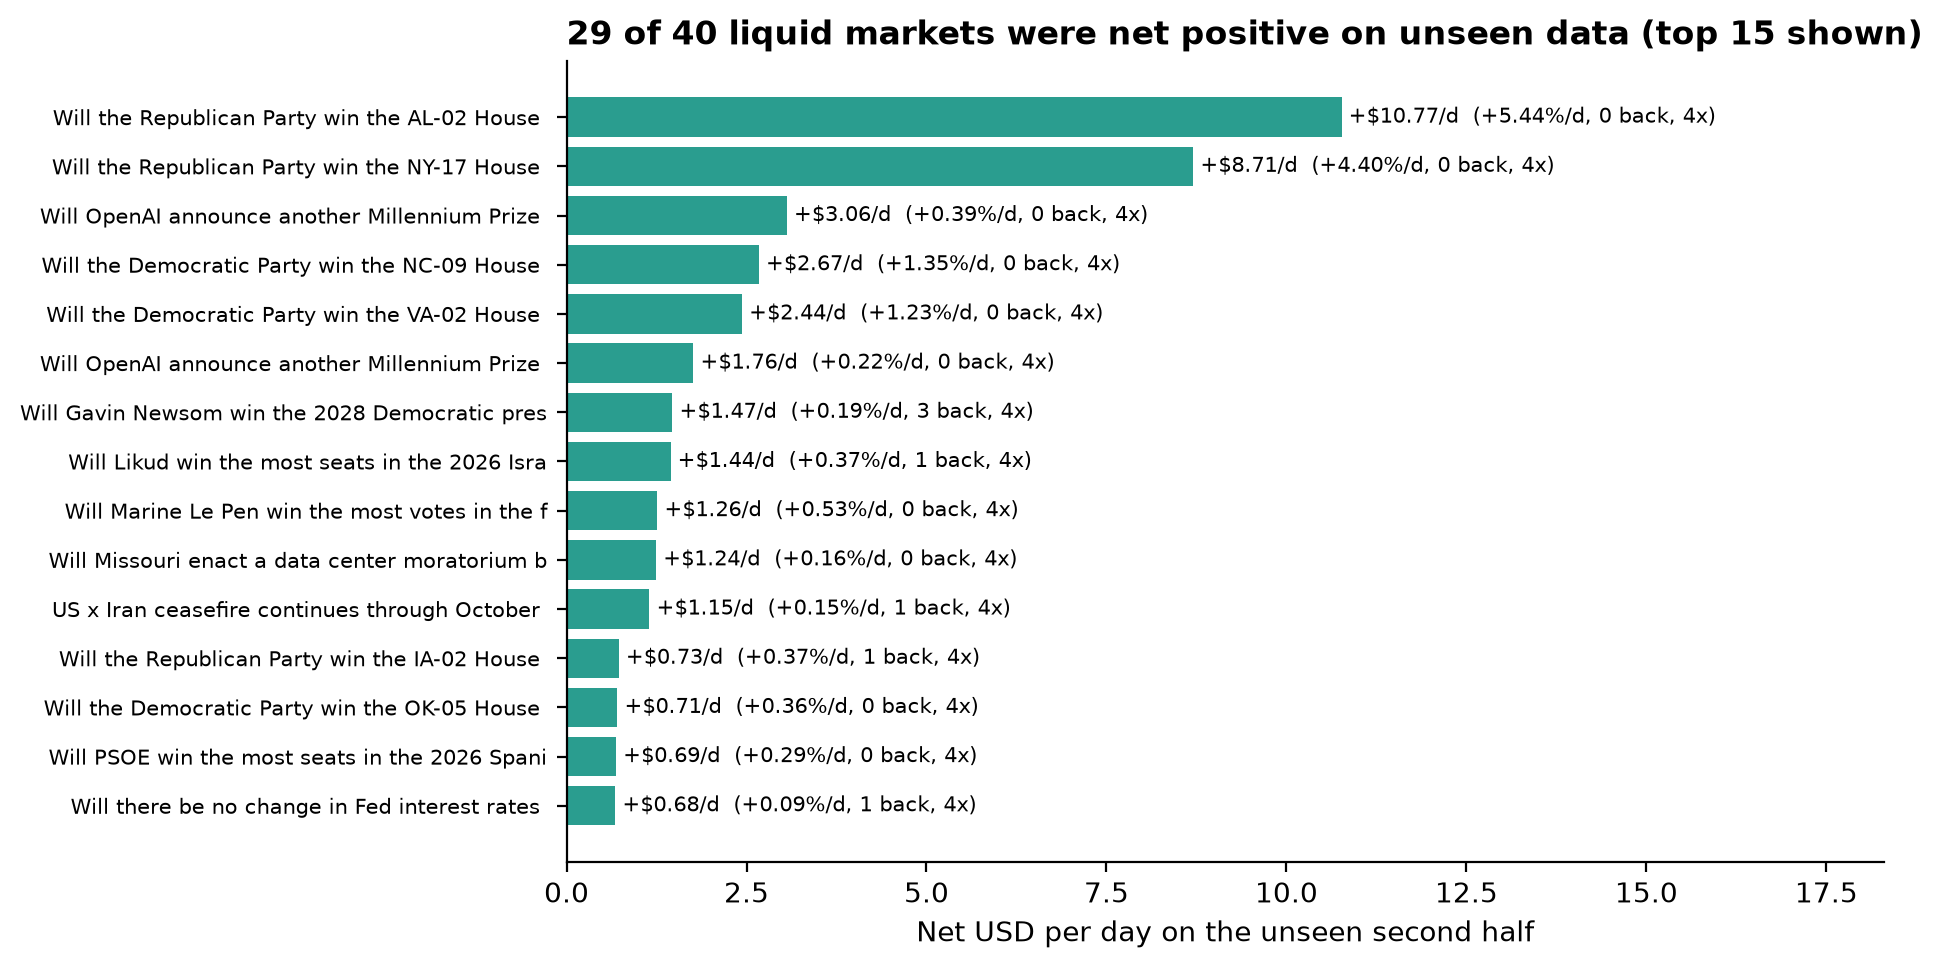
\includegraphics[width=0.92\linewidth]{positive-markets}
\caption{Net per day on the unseen half for the 15 best of the 29 positive markets.}
\end{figure}
\begin{table}[H]\centering\small
\begin{tabular}{@{}lrrr@{}}
\toprule
Group & Markets & Net \$/day & Rate/day \\
\midrule
Markets positive on the unseen half & 29 & +\$44.61 & +0.45\% (on \$9,874) \\
All markets except the three largest losers & 37 & +\$29.00 & --- \\
Median liquid market & --- & +\$0.53 & --- \\
\bottomrule
\end{tabular}
\caption{The 29 were identified after the test, so their combined rate looks back, not forward.}
\end{table}

\subsection{Low-fill settings were positive 95\% of the time}
\begin{figure}[H]\centering
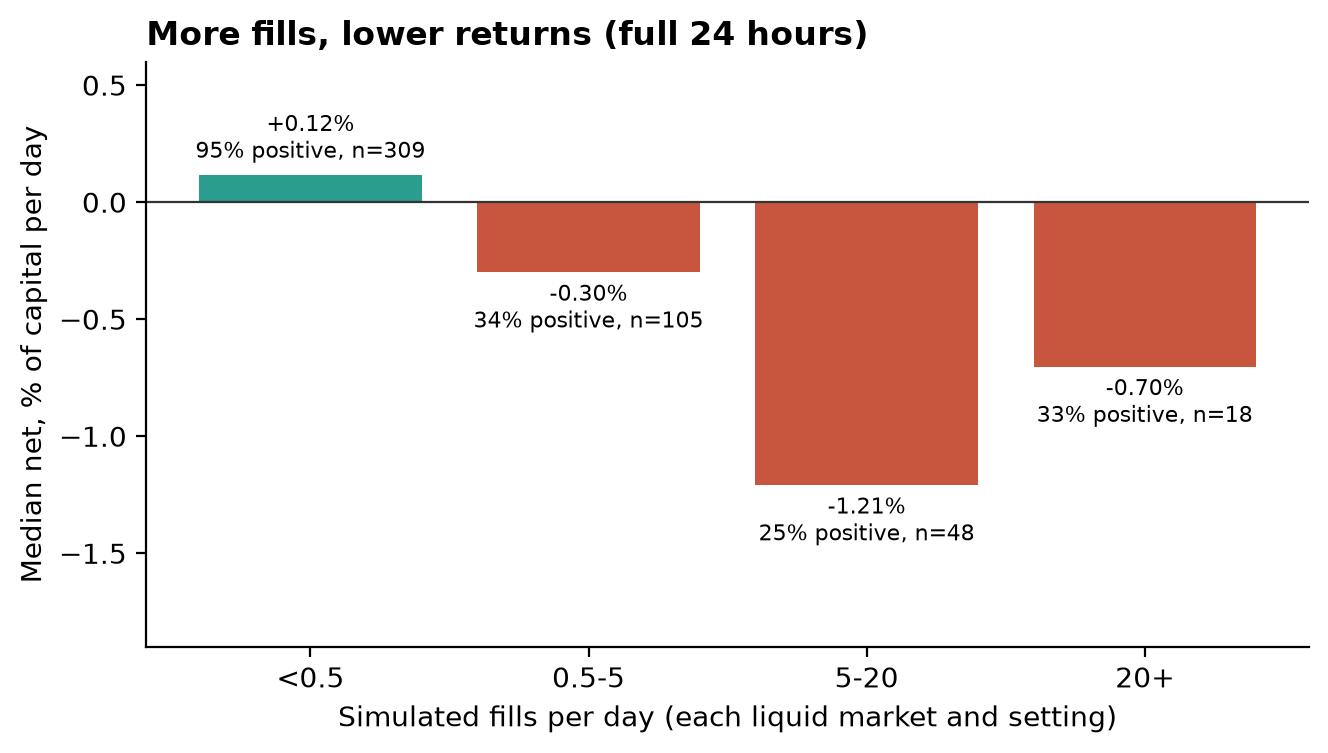
\includegraphics[width=0.78\linewidth]{interaction-final}
\caption{Every liquid market and setting, grouped by simulated fills per day (full 24 hours).}
\end{figure}
Settings that were rarely filled earned a median +0.12\% per day, and 95\% of them were positive (309 combinations). The edge is earning reward while rarely being hit.

\subsection{Small budgets were positive in the capital simulation}
\begin{table}[H]\centering\small
\begin{tabular}{@{}rrrrr@{}}
\toprule
Capital & Markets & Net \$/day & Rate/day & 30 days, compounded \\
\midrule
\$100 & 2 & +\$2.33 & +2.36\% & +101\% (+\$100) \\
\$250 & 4 & +\$2.65 & +1.08\% & +38\% (+\$93) \\
\$500 & 5 & +\$1.11 & +0.24\% & +7\% (+\$34) \\
\$1,000 & 9 & +\$2.67 & +0.28\% & +9\% (+\$83) \\
\bottomrule
\end{tabular}
\caption{Allocations chosen on the first half and scored on the second. Small budgets fund only the top-ranked 2--9 markets; this is a small sample. Larger budgets are covered in Section~\ref{sec:neg}.}
\end{table}

\subsection{Market reach is large}
\begin{figure}[H]\centering
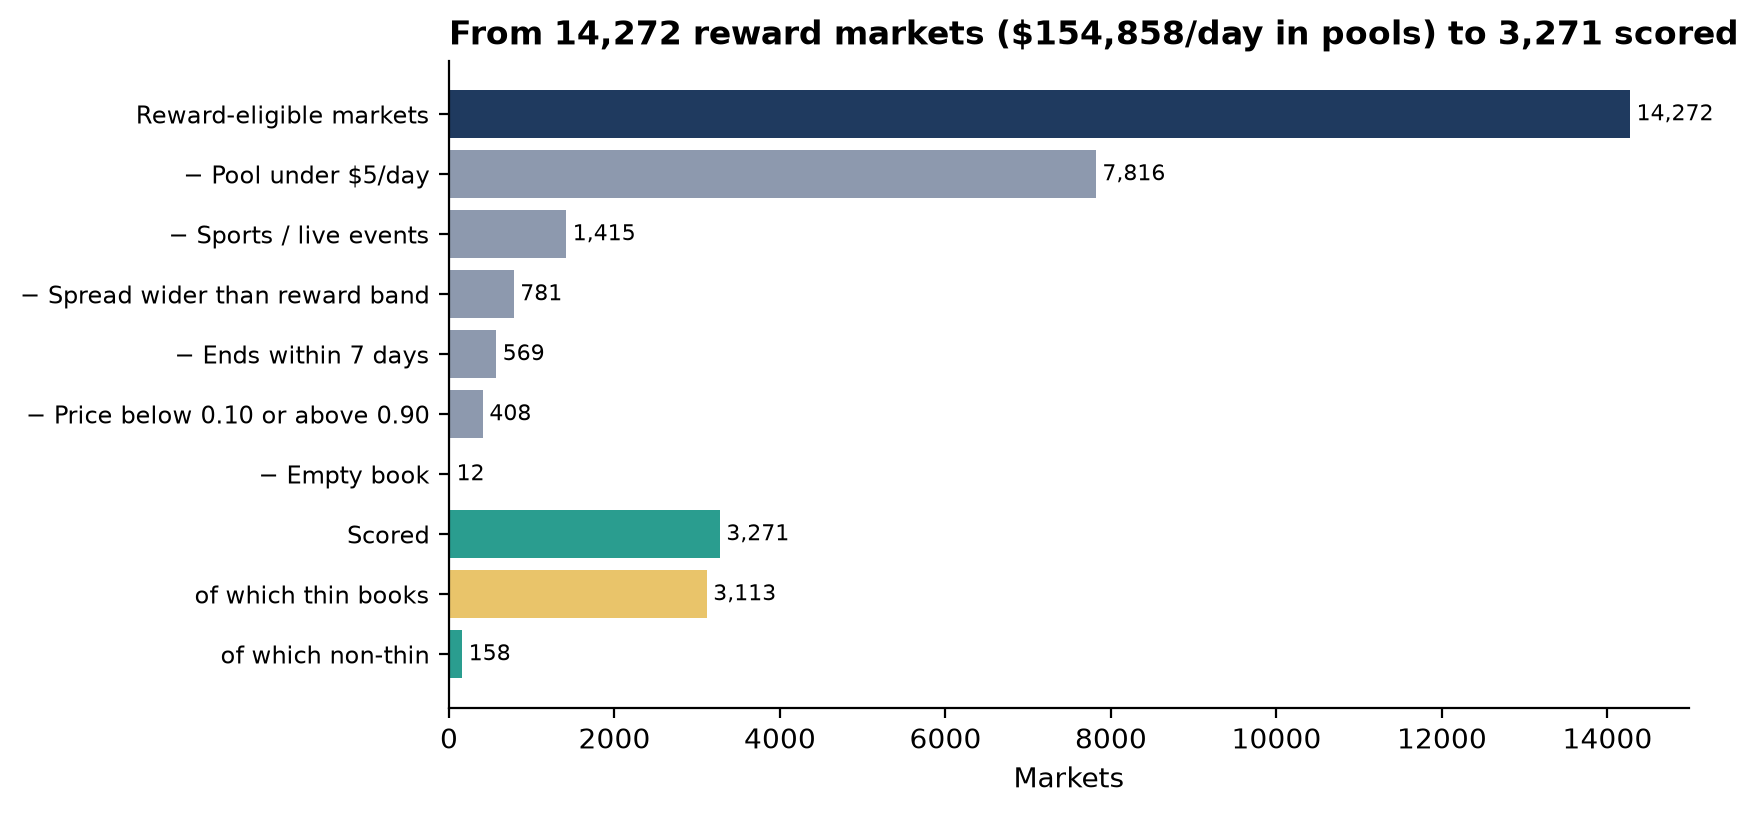
\includegraphics[width=0.85\linewidth]{scan-funnel}
\caption{14,272 reward-eligible markets with \$154,858 per day in pools; 158 liquid markets after filtering.}
\end{figure}

\subsection{Per-\$100 upside scenarios}
\begin{table}[H]\centering\small
\begin{tabularx}{\linewidth}{@{}p{4.2cm}rrY@{}}
\toprule
Scenario & Per \$100/day & 30 days & Basis \\
\midrule
29 positive markets (looking back) & +\$0.45 & +\$14.5 & Unseen-half result of the markets that turned out positive \\
First half (hindsight) & +\$0.40 & +\$12.7 & Settings chosen and scored on the same data \\
Reward only, no fill cost & +\$0.57 & +\$18.6 & Best 10 liquid markets, snapshot \\
\bottomrule
\end{tabularx}
\caption{Upper-bound scenarios. The forward-looking portfolio figure is in Section~\ref{sec:neg}.}
\end{table}

\section{Negative results}\label{sec:neg}
\begin{figure}[H]\centering
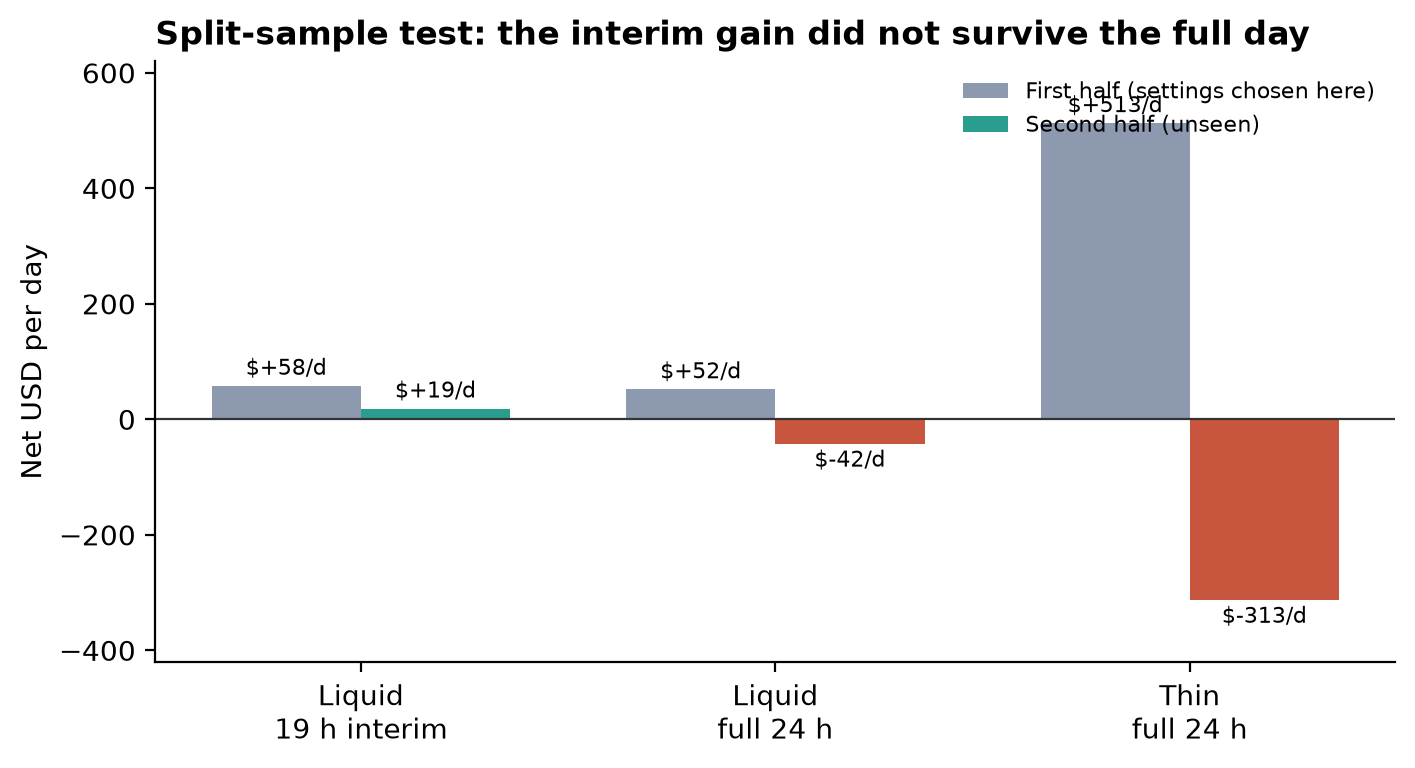
\includegraphics[width=0.8\linewidth]{walkforward-final}
\caption{Split-sample test: the 19-hour interim gain did not survive the full day.}
\end{figure}
\begin{table}[H]\centering\small
\begin{tabular}{@{}lrrrr@{}}
\toprule
Test (net \$/day) & First half & Second half & Capital & Rate \\
\midrule
Liquid, per-market settings (19 h interim) & +\$57.83 & +\$18.54 & \$12,982 & +0.14\% \\
Liquid, per-market settings (full day) & +\$51.83 & $-$\$42.44 & \$12,975 & $-$0.33\% \\
Liquid, size capped at minimum & +\$13.21 & $-$\$10.44 & \$3,183 & $-$0.33\% \\
Liquid, one group setting & +\$4.18 & $-$\$17.87 & \$13,095 & $-$0.14\% \\
Thin books, per-market settings & +\$512.69 & $-$\$312.91 & \$11,308 & $-$2.77\% \\
\bottomrule
\end{tabular}
\caption{Three liquid markets lost \$71.44 per day between them, outweighing the 29 winners.}
\end{table}

\begin{figure}[H]\centering
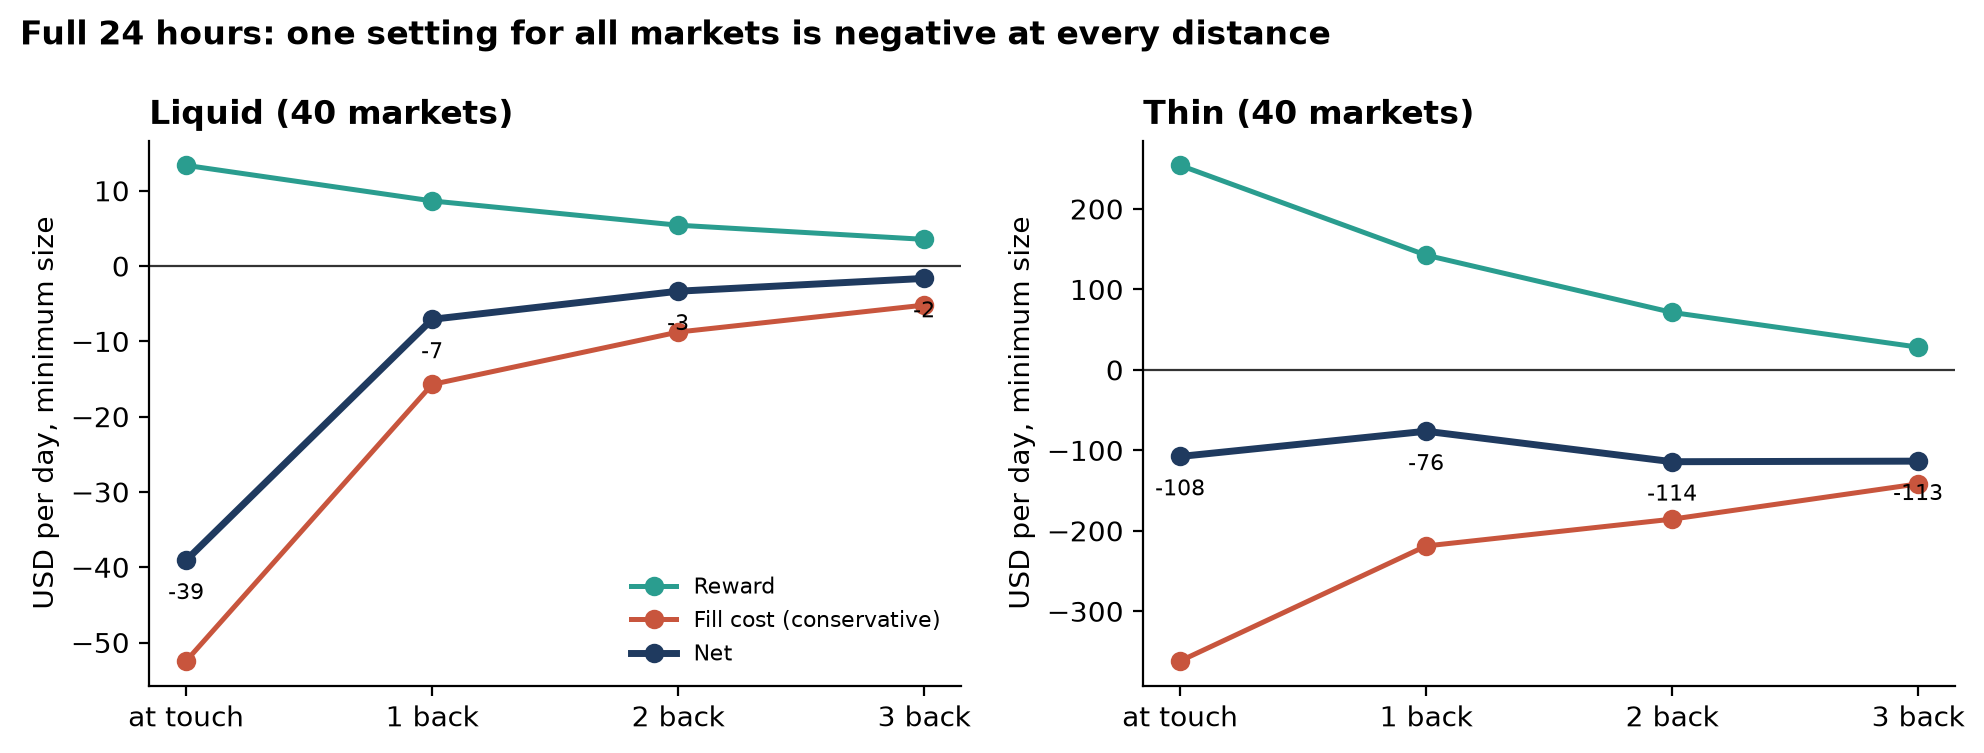
\includegraphics[width=\linewidth]{offset-curves-final}
\caption{One setting for all markets was negative at every quote distance over the full day.}
\end{figure}

\begin{figure}[H]\centering
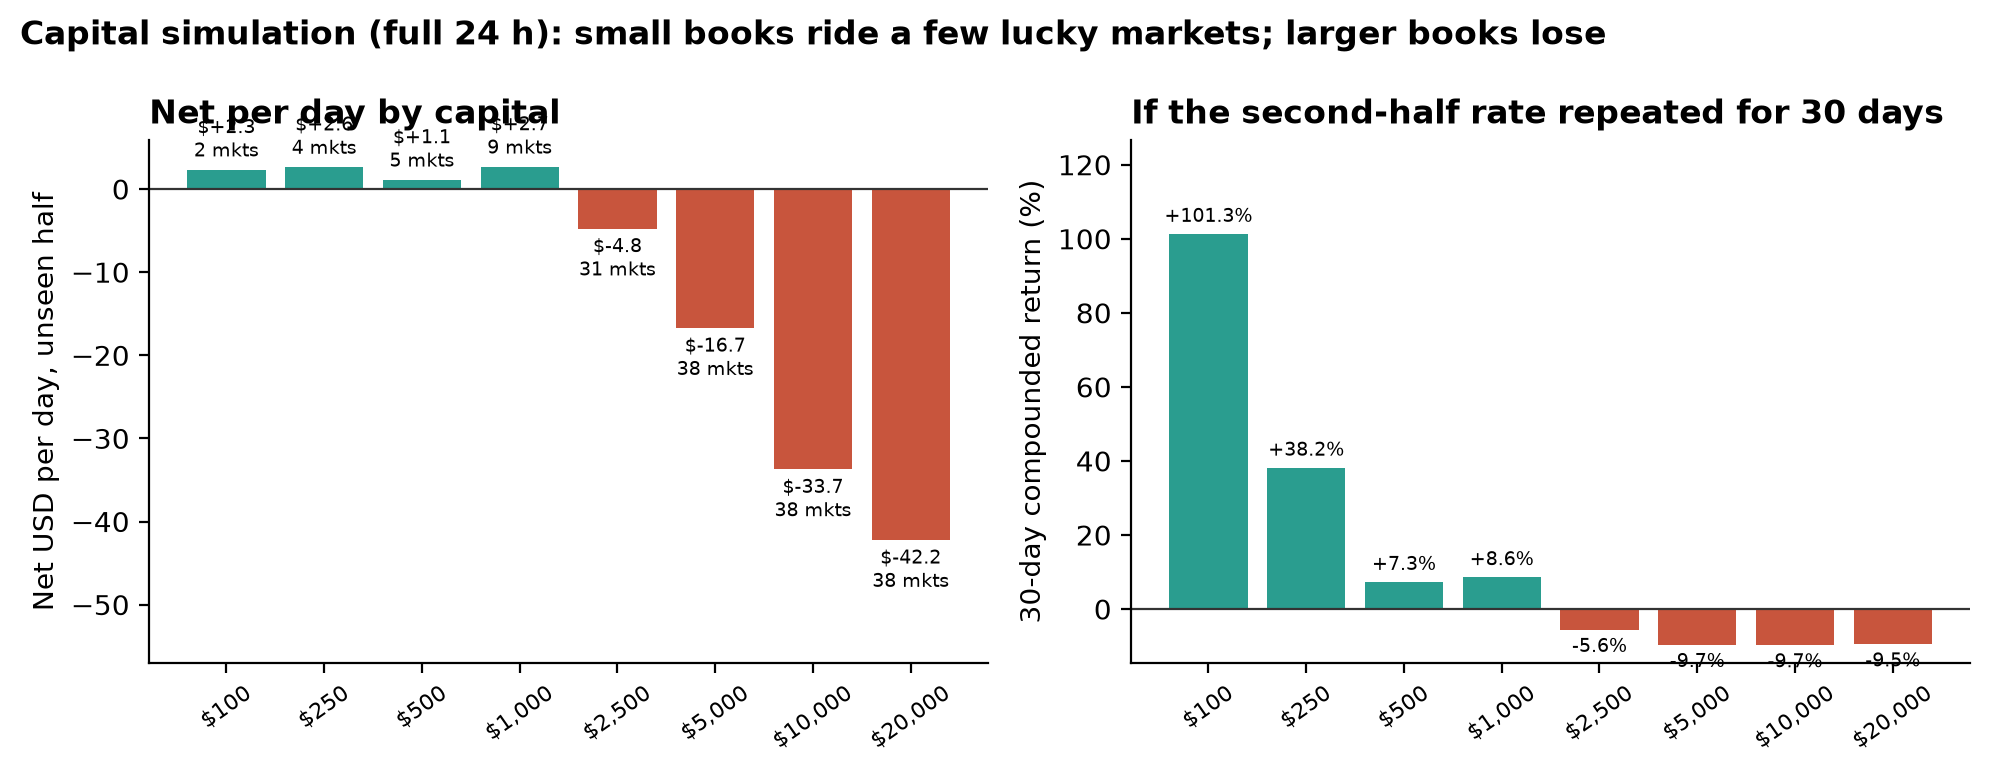
\includegraphics[width=\linewidth]{capital-sim-final}
\caption{Capital simulation: budgets from \$2,500 upward converged on about $-$0.33\% per day.}
\end{figure}
\begin{table}[H]\centering\small
\begin{tabular}{@{}rrrrr@{}}
\toprule
Capital & Markets & Net \$/day & Rate/day & 30 days, compounded \\
\midrule
\$2,500 & 31 & $-$\$4.77 & $-$0.19\% & $-$6\% ($-$\$139) \\
\$5,000 & 38 & $-$\$16.75 & $-$0.34\% & $-$10\% ($-$\$479) \\
\$10,000 & 38 & $-$\$33.74 & $-$0.34\% & $-$10\% ($-$\$964) \\
\$20,000 & 38 & $-$\$42.24 & $-$0.33\% & $-$9\% ($-$\$1,208) \\
\bottomrule
\end{tabular}
\caption{Per \$100, the forward-looking portfolio figure is $-$\$0.33 per day ($-$\$9.33 over 30 days).}
\end{table}

Other negatives: the concluded one-hour paper runs each lost 0.07--0.09\%; thin-book rewards fell from \$414 to \$263 per day as competition rose; and quoting at the touch lost $-$1.13\% per day on liquid markets.

\section{Risks}
\begin{itemize}[leftmargin=1.2em]
  \item \textbf{Tail losses from adverse moves.} A few news-driven moves outweighed a day of reward.
  \item \textbf{Overfitting.} Settings that looked best on one half lost on the other; the interim result overstated performance.
  \item \textbf{Thin and manipulable books.} Projected rewards there did not survive fills.
  \item \textbf{Capacity.} Rewards come from fixed pools (\$5,792 per day across the 40 liquid markets), so returns fall as size grows.
  \item \textbf{Model gaps.} Rewards are projected, queue position is simplified, and benign fills are ignored.
  \item \textbf{Multi-outcome support and access.} Most of the best markets are multi-outcome, which the runner cannot yet quote; eligibility from the operating location is unverified.
\end{itemize}

\section{Gates before real capital}\label{sec:gates}
\begin{warn}
Current status: none of these gates has passed. Each is a condition for a capital decision.
\end{warn}
\begin{enumerate}[leftmargin=1.5em]
  \item Positive net out of sample across several days and splits, with tail losses included.
  \item Jump and news protection that pulls quotes before large moves, tested on recorded data.
  \item The same result from the full paper runner, not only the optimiser.
  \item Multi-outcome quoting implemented and tested; independent auditor updated.
  \item Live-path readiness, eligibility and wallet checks.
  \item Written sign-off on a canary size and stop rules.
\end{enumerate}

\section{Next steps}
\begin{enumerate}[leftmargin=1.5em]
  \item Add a jump filter that pulls quotes on sharp moves or volume spikes, and rerun the split test. This targets the three markets that caused the portfolio loss.
  \item Record further days and test settings chosen on one day against a different day.
  \item Focus the next paper run on low-fill settings in the liquid markets that stayed positive, at minimum size.
  \item Add multi-outcome quoting to widen the pool of liquid markets.
\end{enumerate}

\section*{Reproducibility}
\small
Scan \texttt{scripts/mm-reward-scan.mts}; recording \texttt{scripts/mm-reward-projection.mts} (run \texttt{2026-10-20T18-40-36-481Z}); optimiser \texttt{scripts/mm\_param\_optimiser.py}; split test and capital simulation \texttt{scripts/mm\_walkforward\_capital.py} (outputs in \texttt{final-20261021/}); benchmark and fixes in \texttt{docs/}.

\end{document}
